\svnkwsave{$RepoFile: siminos/spatiotemp/chapter/reportRJ.tex $}
\svnidlong {$HeadURL: svn://zero.physics.gatech.edu/siminos/spatiotemp/chapter/reportRJ.tex $}
{$LastChangedDate: 2020-05-07 17:34:06 -0400 (Thu, 07 May 2020) $}
{$LastChangedRevision: 7184 $} {$LastChangedBy: predrag $}
\svnid{$Id: reportRJ.tex 7184 2019-12-12 06:24:59Z predrag $}

\chapter{Frequencies of Cat Map Winding Numbers}
% {Rana's research report}
\label{chap:reportRJ}
\renewcommand{\cl}[1]{{\ensuremath{n_{#1}}}}   % discrete length of a cycle, Predrag



\noindent
{\Large{\textbf{Rana Jafari Summer 2016 Report}}}


\section{Introduction}
\label{sect:introRepJR}

                %     \PC{2016-11-04}{copied to GHJSC16
The linear mapping $A$ on unit 2-torus is defined as follows:
$$ A = \left (
\begin{array}{cc}
a & 1 \\
ab -1 & b \\
\end{array}
\right ) $$
\beq
\left (
\begin{array}{c}
q_{t+1} \\
p_{t+1} \\
\end{array}
\right ) = A \left (
\begin{array}{c}
q_t \\
p_t \\
\end{array}
\right ) \quad  \mod\: 1
\ee{RSCatMap}
Such `toral automorphisms' provide very simple examples of chaotic
Hamiltonian dynamical system. The unit determinant results in measure
preservation, and $|\Tr (A) |> 2$ in hyperbolicity. We shall refer to the
$s=3$ case as the `Arnol'd cat map' (also known as the Arnol'd-Sinai cat
map\rf{ArnAve,deva87}), and to cases where integer $s>3$  as `cat maps'.
The integers obtained by taking modulo 1 can be interpreted as winding
numbers\rf{Keating91}. Rational and irrational initial coordinates
generate periodic and  ergodic orbits, respectively. The properties of
periodic orbits are studied in detail  by Percival and
Vivaldi\rf{PerViv87b}.
The initial part of this report focuses on finding the frequencies of
winding numbers generated by the iterations of map \refeq{RSCatMap} for
different integer values of $s=\Tr A$. These frequencies enable us to
find the areas of partitions in phase space corresponding to words of
symbolic dynamics of Arnol'd cat map. In \refsect{sect:RJCouplCatMaps}
we apply these methods to computation of the frequencies of symbol
patterns for \catlatt s.

\section{Numbers of periodic orbits}
\label{sect:NoPOs}


% RJpost{2016-05-20

The number of period-\cl{} periodic points of the $[2\!\times\!2]$
matrix transformation ${\bf A}$ on a unit torus $[0,1)\times[0,1)$, is
equal to number of fixed points of transformation ${\bf A}^\cl{}$.
    \PC{2016-08-03}{refer to where this is proven, or derive this statement here?}
We can find this number by solving:
\begin{equation}
{\bf A}^\cl{}{\bf x}_0 = {\bf x}_0 \quad \mod 1
\label{RSCattyMap}
\end{equation}

$$ \Rightarrow ({\bf A}^\cl{} - {\bf I} )\ {\bf x}_0 = {\bf v}
$$
where ${\bf v } $ is an integer valued column vector.
%%This implies,
%%$$ {\bf A}^\cl{}-I \ (mod \ 1) = 0$$
%%which is trivially satisfied.\\ \\
The number of solutions to
\refeq{RSCattyMap}
is equal to $|\det({\bf A}^\cl{} - {\bf I} )|$. Since the $({\bf A}^\cl{} - {\bf I} ){\bf x}_0 $
transforms unit square to parallelogram with area
$|\det({\bf A}^\cl{} - {\bf I} )|$,
the parallelogram covers the unit square
$|\det({\bf A}^\cl{} - {\bf I} )|$ times.
By direct calculation, or by the $[2\!\times\!2]$  matrix identity
\[
\det( {\bf A} + {\bf B}  ) = \det({\bf A}) + \det( {\bf B} ) + \tr ({\bf A}) \ \tr ({\bf B}) - \tr ({\bf A} {\bf B}),
\]
together with $ \det({\bf A}^\cl{})=\left(\det({\bf A})\right)^\cl{} = 1 $:
$$\det( {\bf A}^\cl{} -{\bf I} )
= \det({\bf A}^\cl{}) + \ 1\ + (-2) \ \tr ({\bf A}^\cl{}) \   - \tr ( - {\bf A}^\cl{}) $$
Hence
the number of periodic points is
\beq
N_\cl{} =  |\tr ({\bf A}^\cl{})\ - \ 2\ |
 = | \Lambda^\cl{} + \Lambda^{-\cl{}} -\, 2\, |
 \,.
\label{RSNoPerPoints}
\eeq
where $\Lambda$ is the larger eigenvalue of ${\bf A}$.

For the Arnol'd cat map
\[
{\bf A}= \left (
		\begin{array}{cc}
		1&1\\
		1&2\\
		\end{array} \right)
\,,
\]
the powers of $ {\bf A}$ are given by the Fibonacci numbers
    \PC{2016-05-21}{to RS and AKS make this into an exercise,
        write up the solution}
$${\bf A}^n\ = \ \left (
		\begin{array}{cc}
		F_{2n - 1}&F_{2n}\\
		F_{2n}&F_{2n+1}\\
		\end{array} \right)$$
with seed values  $ F_1 = 1,\; F_2 = 1 \,.$
Therefore,
$$ N_\cl{} =  F_{2\cl{} - 1}+F_{2\cl{}+1}  - 2 $$
For example
\bea
N_1 &=& F_{1}+F_{3}  - 2 = 1+2-2 = 1
\continue
N_2 &=& F_{3}+F_{5}  - 2 = 2+5-2 = 5
\,,\qquad \cdots
\label{RJN1N2}
\eea


\subsection{Keating's counting of periodic points}

Keating\rf{Keating91a} derives the number of periodic points of the cat
map as follows:

The $(q_j,p_j)$ periodic point of period $n$ satisfy
\begin{equation}
 \left (
		\begin{array}{c}
		q_{fixed}\\
		p_{fixed}\\
		\end{array} \right) \ = \ (A^n \ - \ I \ )^{-1} \
 \left (
		\begin{array}{c}
		m\\
		n\\
		\end{array} \right)
\label{FixedPointsEq}		
\end{equation}		
``where m and n are integers which correspond to the winding numbers of
the associated point $( q_{fixed},\ p_{fixed})$ around the torus under
the action of the map $A$. For this point to have coordinates between 0
and 1, m and n must lie within the parallelogram formed by the action of
the matrix $(A^n \ - \ I \ )^{-1}$ on the unit square. We call this the
fundamental parallelogram associated with $A^n$. It tessellates the plane
in which the (integer) lattice of winding numbers $(m,\ n)$ lies. Hence
the number of fixed points of $A^n$ is given by its area, which is
$\det(A^n \ - \ I ) = \tr(A^n)\ -\ 2$. It may be seen from
\refeq{FixedPointsEq} that these fixed points form a lattice in phase
space."

\section{Relative frequencies of cat map words}


In this section we evaluate the number of times that a symbol appears in the
symbolic sequence of an ergodic orbit of a cat map.  The
Arnol'd cat map alphabet consists of 4 letters
$ \mathcal{A} =  \{ \underline{2}, \underline{1}, 0, 1\} $.  $
\mathcal{A}$ is obtained from the equation of motion:
\begin{equation}
q_{n-1} - 3 q_{n} + q_{n+1} = m_{n},  \ \ \  m_{n} \in  \mathcal{A}
\end{equation}
For notational convenience, in alphabets we shall denote negative
$m$ by underlining them, \ie,
\(
\{ \underline{2}, \underline{1}, 0, 1\} = \{ -{2}, -{1}, 0, 1\}
\,.
\)
To find $p(m)$, the relative frequency of symbol $m$, a Python program was written in
which $100$ arbitrary initial points are iterated for $n \ = \ 500000$
times. After each iteration,  the obtained symbols are stored in an array
of length  $n$, and four counter variables are used to find how many
times a symbol appears in the sequence.  Finally, the average of
number of repetitions for each symbol is found. Dividing these averages
by $n$ gives the frequency of each symbol.
The final result is
\[
p(\underline{2}) \ = \  0.16670, \ p(\underline{1}) \ =  \ 0.33328, \ p(0) \ =  \ 0.33333, \ p(1) \ = \ 0.16669
\]
Next, we look for the relative frequency of $- m_{i} m_{i+1} -$, $p(m_{i}
\ m_{i+1})$. To find $p(m_{i} \ m_{i+1})$, a function is added to the
previous program which checks the next symbol of each item of array, and
then, increments the corresponding counter. The relative frequencies of
the four symbols with $4^2$ combinations (for \prune{s_{i} s_{i+1}} ) are
listed in \refTab{tab:RJ2letFreq}.
\refTab{RJpruning} lists $N_n$, the total number of pruned blocks of
length  $n=\cl{a}$, and $\tilde{N}_n$, the number of new pruned blocks of
length  $\cl{a}$, with all length  $\cl{a}$ blocks that contain shorter
pruned blocks already eliminated.

\par
The relative frequencies can be obtained analytically by eliminating two
coordinates corresponding to  2-symbol from the equations of motion.
Excluding two coordinates from the equations of motion and applying
boundary conditions ($ 0 \leq q < 1$) gives the following inequalities
for 2-symbol words $- m_{i} m_{i+1} -$:
\bea
0 &\leq& \frac{1}{8}(-3 m_{i} -m_{i+1}+3 x_{1} + x_{2}) <1,
\continue
0 &\leq& \frac{1}{8}(- m_{i} -3 m_{i+1}+ x_{1} + 3 x_{2}) <1.
\label{2symbolinequalities}
\eea
The areas of regions confined by these inequalities represents the relative frequencies corresponding to each 2-symbol word (\reftab{tab:RJ2letFreq}).
\refFig{RJfrequencies} shows the analytically found frequencies of words with lengths 1 to 6.

\begin{table}
\begin{center}
\begin{tabular}{ c|cccc }
 & $\underline{2}$ & \underline{1} & 0 & 1\\
  \hline
 $\underline{2}$ &  0  & 0.0208 &  0.0625 &  0.0833\\
 \underline{1} &  0.0209 &  0.125 &  0.125 &  0.0625 \\
 0 & 0.0625 & 0.125 & 0.125 &  0.0209\\
 1 & 0.0833 & 0.0625 &  0.0209 &  0\\
\end{tabular}
=
\begin{tabular}{ c|cccc }
 & $\underline{2}$ & \underline{1} & 0 & 1\\
  \hline
 $\underline{2}$ &  0    & 1/48 &  1/16 &  1/12\\
 \underline{1} &  1/48 &  1/8 &  1/8 &  1/16 \\
  0 &  1/16 & 1/8  &  1/8 &  1/48\\
  1 & 1 /12 & 1/16 &  1/48 &  0\\
\end{tabular}
\end{center}
  \caption{\label{tab:RJ2letFreq}
The relative frequencies of 2-symbol words \prune{m_{i} m_{i+1}} for
the Arnol'd cat map, obtained (left) from a long-time numerical simulation,
(right) analytically.
% with $4^2$ combinations
Column: \ $m_{i}$.  Row: \ $m_{i+1}$.
There is only one pruning rule: \prune{11} is pruned. By the reflection
symmetry, also \prune{\underline{2}\underline{2}} is pruned. As defined by
\refeq{2symbolinequalities}, these frequencies are rational numbers, and
their sum is 1.
  }
\end{table}



\begin{table}
\begin{center}
            \begin{minipage}[t][][b]{0.33\textwidth}
            \begin{center}
\begin{tabular}{r|r|r}
  % after \\: \hline or \cline{col1-col2} \cline{col3-col4} ...
  $\cl{a}$ & $N_n$ & $\tilde{N}_{n}$ \\
  \hline
  2 & 2 & 2 \\
  3 & 22 & 8 \\
  4 & 132 & 2 \\
  5 & 684 & 30 \\
  6 & 3164 & 2 \\
  7 & 13882 &   \\
  \\
\end{tabular}

    (a)
            \end{center}\end{minipage}
~~~~~~~
            \begin{minipage}[t][][b]{0.33\textwidth}
            \begin{center}
\begin{tabular}{r|r|r|}
  % after \\: \hline or \cline{col1-col2} \cline{col3-col4} ...
  $\cl{a}$ & $N_n$ & $\tilde{N}_{n-1}$ \\
  \hline
  2 & 2 & 0 \\
  3 & 22 & 2 \\
  4 & 132 & 8 \\
  5 & 684 & 2 \\
  6 & 3164 & 30 \\
  7 & 13894 & 2 \\
  8 & 58912 & 70 \\
  9 & 244678 & 16 \\
  10 & 1002558 & 198 \\
  11 & 4073528 & 2 \\
  12 & 16460290 & 528 \\
  13 &   & 2 \\
\end{tabular}

(b)
            \end{center}\end{minipage}
\end{center}
	\caption{\label{RJpruning}
$N_n$ is the total number of pruned blocks of length  $n=\cl{a}$ for the Arnol'd
cat map, $s=\tr[A]=3$. $\tilde{N}_n$ is the number of new pruned blocks
of length  $\cl{a}$, with all length  $\cl{a}$ blocks that contain shorter pruned
blocks already accounted for.
(a) Computation carried in this report.
(b) Numbers obtained by Li Han (unpublished). Note that (empirically)
there is a single new pruning rule
for each prime-number period (it is listed as 2 rules, but
by the reflection symmetry there is only one).
    }
\end{table}


\begin{figure}
	\centering
	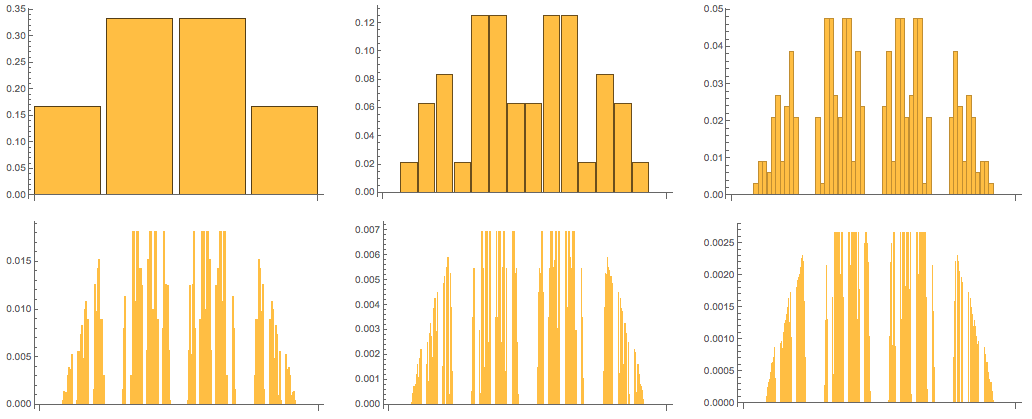
\includegraphics[width=0.95\textwidth]{RJfrequencies}
	\caption{\label{RJfrequencies}
Frequencies of words of symbols. (Left to right: sub sequences of length
1, 2, 3, ..., 6.)
            }
\end{figure}



\subsection{Numerical computations}

To find all the possible periodic lengths of initial sets, $\{q_1, q_2\}
= \{\frac{P_1}{N},\frac{P_2}{N}\}$, we can consider the initial points to
be $(P_1, P_2)$ on $ [0, \ N)^2$, and, following  \refref{BaoYan12},
after each iteration we take $\mod N$. In this way, we use only s
integers, and, after each iteration the output is exact, with no floating
point round-off errors.
The periods that we obtain for the lowest values of $N$ are as follows:
\par for $\{q_1, q_2\} = \{\frac{P_1}{10},\frac{P_2}{10}\} \ : T \in \{1,\ 2,\ 3, \ 6, \ 10, \ 30\}$,
\par for $ \{q_1, q_2\} = \{\frac{P_1}{100},\frac{P_2}{100}\} : T \in \{1, \ 2, \ 3, \ 6, \ 10, \ 30, \  50, \ 150\}$
\par for $\{q_1, q_2\} = \{\frac{P_1}{8},\frac{P_2}{8}\} : T \in \ \{1, \ 3, \ 6\}$
\par for $\{q_1, q_2\} = \{\frac{P_1}{17},\frac{P_2}{17}\} : T \in \{1, 18\}$


\subsection{Entropy}

\begin{figure}	
	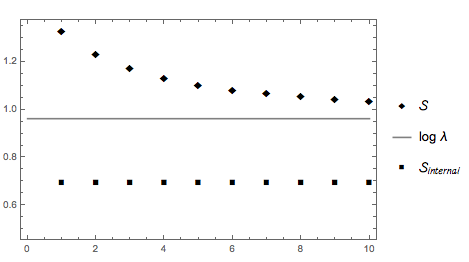
\includegraphics[width=0.65\textwidth]{RJentropyPlot}
	\caption{\label{fig:RJentropyPlot}
Entropies $\mathcal{S}$ and $\mathcal{S}_{internal}$
vs. the length $\cl{a}$ of \po s used to estimate them.
    }
\end{figure}


Given the frequencies $p(a)$ with which a blocks
$ a = a_1 a_2 ...\ a_{\cl{a}}$ occur, the sum
\beq
\lim_{\cl{a}\to\infty} -\,\frac{1}{\cl{a}} \sum_{a}{p(a) \log{p(a)}}\ = - \log \Lambda
\,,
\ee{EntropyEigenvalue}
where $ \Lambda = \frac{3 - \sqrt{5}}{2} $ is the eigenvalue of  $ \bf{A} = \left (
		\begin{array}{cc}
		1&1\\
		1&2\\
		\end{array} \right) $.
\par
Evaluating
\beq
\mathcal{S} =  -\,\frac{1}{\cl{a}} \sum_{a}{p(a) \log p(a)}
\ee{EntropyValue}
for $\cl{a} = 1$ to $10$ gives the values listed in \reftab{tab:RJentropies}.
Excluding all sequences that contain the external symbols and evaluating
$\mathcal{S}$ for the remaining pure  $\{ \underline{1},0\}$ sequences gives the exact,
complete symbolic dynamics expression (B. Gutkin, unpublished)
\[
\mathcal{S}_{internal} =  -\,\frac{1}{\cl{a}} \log \frac{1}{2^{\cl{a}}} = \log 2
\,,
\]
which we verify numerically in \reffig{fig:RJentropyPlot}.


%%%%%%%%%%%%%%%%%%%%%%%%%%%%%%%%%%%%%%%%%%%%%%%%%%%%%%%%
\begin{table}
\begin{center}
\begin{tabular}{ r|c|c}
 $\cl{a}$& $\mathcal{S}$& $\frac{ \mathcal{S}-\log \Lambda }{\log \Lambda}$\\
   \hline
1& 1.3297 & \%38.1 \\
 2 &  1.2348 &  \%28.3\\
 3 & 1.1731 &\% 21.9\\
 4 & 1.1337 & \%17.8 \\
 5& 1.1051 &\%14.8 \\
 6& 1.0843 &\%12.7 \\
 7& 1.0682 &\%11.0\\
 8& 1.0558 & \%9.71\\
 9& 1.0458 &\%8.67 \\
 10& 1.0378 &\%7.83 \\
\end{tabular}
\end{center}
  \caption{\label{tab:RJentropies}
Entropies \refeq{EntropyValue} for strings of lengths
$\cl{a} = 1$ to $10$, $s = 3$ Arnol'd cat map.
  }
\end{table}
%%%%%%%%%%%%%%%%%%%%%%%%%%%%%%%%%%%%%%%%%%%%%%%%%%%%%%%%%%%


\section{{\catLatt}}
\label{sect:RJCouplCatMaps}

In the {\catlatt}, ``particles'' (\ie, a cat map at each lattice site)
are coupled together by the next-neighbor coupling rules:
\[
q_{n, t+1}=p_{n,t}+(s-1)q_{n,t} - q_{n+1,t} - q_{n-1,t} - {m}^q_{n,t+1}
\]
\[
p_{n,t+1}= p_{n,t} + (s-2) q_{n,t} - q_{n+1,t} - q_{n-1,t} - {m}^p_{n,t+1}
\]
The symbols of interest can be found by:
\[
m_{n,t} = q_{n,t+1} + q_{n,t-1} + q_{n+1,t} + q_{n-1, t} -  s \, q_{n,t}
\,.
\]
The results presented in this section are obtained by simulations. In
order to make the computation exact, the denominators and numerators of
the coordinates are stored as integers, \ie, only integers are used in all
calculations presented here.

\subsection{Frequencies of symbols}

The obtained relative frequencies for different values of parameter $b$ in
    \PC{2016-11-03}{
    Where did the $c$ come from? Shouldn't it be $c=-1$ by area preservation?
    Oh, I see - it has to do with coupling between sites\rf{GutOsi15}.
    }
\[
A
= - \frac{1}{c}\left( \begin{array}{ll}
       a &1\\
       ab-c^2 & b
       \end{array} \right)
\]
(where $ s= \tr A =a+b $) shows the existence of 6 external and $s-3$
internal symbols from the alphabet $\mathcal{A} =  \{-s+1, -s, ..., 2,
3\} $. The numerical results were close to the expected values, which are $
p(3)= \ p(-s+1) = \ \frac{1}{4!}, \ p(2) = \ p(-s+2)= \ \frac{1}{2} $,
and \ $p(1)= \ p(-s+3) = \ 1-\frac{1}{4!}$ (the relative frequency of an
internal symbols is $1$).

The results of \refTab{freqDiffParNum1} and \refTab{freqDiffParNum2},
suggest that the frequencies are independent of $n$, the number of
particles. Also, the values in \refTab{NormalizationFactor} suggest that
the normalization factor $N$ is expected to be ${1}/{s}$. These
values agree with the analytical values derived for the internal and
external sequences:\\
$$ \frac{1}{N} \left[ 6 \left( \frac{1}{4!}+(1-\frac{1}{4!})+\frac{1}{2}\right) + (s-3)(1) \right] = 1$$
$$\Rightarrow N = s$$
    \PC{2016-12-20}{I do not get $N = s$ from this formula...}

\begin{table}
\begin{center}
\begin{tabular}{c|c|c|c|c|c|c|c|c|}
$n $& $\underline{3}$& $\underline{2}$ & $\underline{1}$ & $0$ & $1$ & $2$ & $3$ & $N$ \\
   \hline
$3$ & $0.04169$ & $0.49896$ & $ 0.96169$ & $1$ & $0.97298$ & $0.49965$ & $0.04116$ & $4.016$\\
 $7$ &  0.04062 & 0.50008 &   0.95917 &  1&  0.95131 &  0.50284 &  0.04054 & 3.995 \\
 $10$ & $0.04127$ &  $0.50135$ &  $0.96255$ &  $ 1$  & $ 0.96019$ & $0.50066$ & $ 0.04178$&$4.007$\\
 $20$ &$0.04120$ & $ 0.50256$ & $ 0.95779 $ & $ 1$ & $0.95871$ & $0.50171$ &  $0.04087$ & $4.003$\\
 \hline
  % 0.04218743,  0.49865395,  0.95819233,  1.        ,  0.95456348,
     %   0.49967509,  0.04212836%
\end{tabular}
\end{center}
\caption{\label{freqDiffParNum1}
$s=4$. Numerically, the relative frequencies of symbols $\underline{1}, 0$ and $1$
are close to 1.
}
\end{table}


\begin{table}
\small{
\begin{center}
\begin{tabular}{ |c|c|c|c|c|c|c|c|c|c|c|c|c|}
 \hline
 $n $&$\underline{7}$&$\underline{6}$&$\underline{5}$&$\underline{4}$ & $\underline{3}$& $\underline{2}$ & $\underline{1}$ & $0$ & $1$ & $2$ & $3$ & $N$\\
   \hline
$3$ & 0.0417&  0.4996 &  0.9560 &  1.  &  0.9961 &  0.9993 & 0.9980 &  0.9974 &  0.9535 & 0.4982 &  0.0414 & 7.981\\
 \hline
 $10$ & 0.0414 &  0.4994  &  0.9535 & 0.9942 &  0.9978 &   0.9902 &  0.9938 &  1. & 0.9551 & 0.49881 &  0.0411 & 7.965\\
  \hline
 $20$ &  0.0410 &   0.5017& 0.9442 & 0.9839 &  0.9916& 0.9837 &  1 &  0.9795 & 0.9576 &  0.4887& 0.0419 & 7.980\\
  \hline
\end{tabular}
\end{center}
\caption{\label{freqDiffParNum2}
$s = 8$. Numerically, the relative frequencies of symbols $\underline{4}, \ \underline{3}, \
\underline{2}, \underline{1}, 0$ and $1$ are close to 1.
}
}
\end{table}


\begin{table}
\begin{center}
\begin{tabular}{ |c|c|}
 \hline
 $s $& $N$\\
   \hline
   5 & 5.0004\\
   \hline
    6 & 5.9988\\
   \hline
   7 & 7.0101\\
   \hline
   8 & 8.0014\\
   \hline
   9 &8.9946\\
   \hline

\end{tabular}
\end{center}
\caption{\label{NormalizationFactor}
    $N$, he normalization factor of relative frequencies.
        }
\end{table}

\subsection{Frequency of blocks of length two}

Next, we look for frequencies of blocks of length 2. These
blocks can be formed by two consecutive symbols of one particle
(e.g. $m_{n,t} m_{n,t+1}$ ) or symbols corresponding to two different
particles at time $t$ (e.g $m_{n,t} m_{n+1,t}$). Based on the results, there is a
symmetry between symbols for a particle (\reffig{RJsymbolsOneParticle}), and
symbols at time $t$ for two different particles (\reffig{RJsymDiffPrc}) (with the
same normalization factor, $N \approx 15 $).

\begin{figure}
	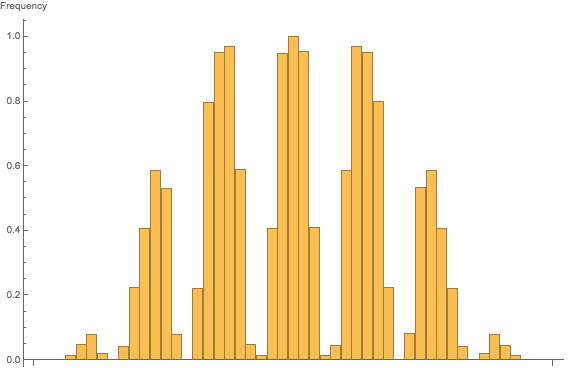
\includegraphics[width=0.65\textwidth]{RJsymbolsOneParticle}
	\caption{\label{RJsymbolsOneParticle}
Relative frequencies of two symbols for a particle ($m_{n,t} m_{n,t+1}$). $s = 4$.
            }
\end{figure}

\begin{figure}

	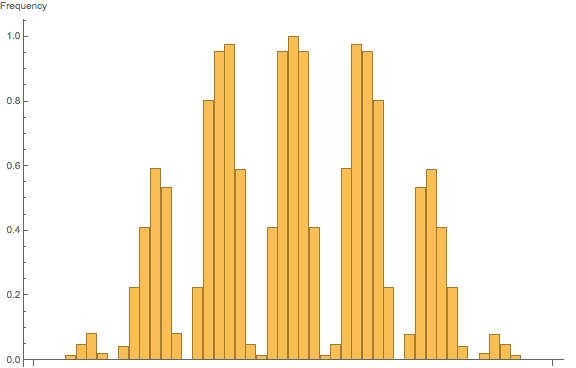
\includegraphics[width=0.65\textwidth]{RJsymDiffPrc}
	\caption{\label{RJsymDiffPrc}
Relative frequencies of two symbols at time $t$ for two different
particles ($m_{n,t} m_{n+1,t}$). $s = 4$.
            }	
\end{figure}

The only pruned blocks for both cases are $ \underline{3}\underline{3} $ and $ 33 $, which is in agreement with the analytical results obtained by simplifying the  inequalities of both cases in Mathematica (which implies that the confined area between the hyper planes is zero):
$$ 0 \leq \frac{1}{15} \left(-4 a_1-a_2+4 x_1+x_2+x_3+x_4+4 x_5+4 x_6\right) < 1,$$
$$ 0 \leq \frac{1}{15} \left(-a_1-4 a_2+x_1+4 x_2+4 x_3+4 x_4+x_5+x_6\right) <1. $$
According to the simulations, the sum of volumes confined between these planes should be 15.

\begin{table}
\begin{center}
\begin{tabular}{ |c|c|}
 \hline
 $s$ & $N$\\
 \hline
 4 & 14.9168\\
 \hline
5 & 23.8374\\
\hline
 6 & 34.8851\\
 \hline
 7 & 48.1024\\
 \hline
 \end{tabular}
\end{center}
 \caption{\label{TwoSymbolsNormalization}
 Normalization factor, $N$, for different values of$s$.
        }
 \end{table}

The  normalization factors, $N$, for different values of $s$ are shown in
\refTab{TwoSymbolsNormalization}. By comparing these values with
inequalities obtained by excluding 2 coordinates corresponding to 2
symbols, it is observed that the normalization factors appear in
equalities as the biggest common denominator. For example, for $s=5$
we have the following inequality:
$$0 \leq \frac{1}{35} \left(-6 a_1-a_2+6 x_1+6 x_2+x_3+x_4+x_5+6 x_6\right) < 1,$$
$$0 \leq \frac{1}{35} \left(-a_1-6 a_2+x_1+x_2+6 x_3+6 x_4+6 x_5+x_6\right) < 1$$
The normalization factor obtained from simulations is approximately 35.

\subsection{Frequencies of  $[2\!\times\!2]$ spatiotemporal domains}

Frequencies of  $[2\!\times\!2]$ spatiotemporal domains of 20 coupled particles
for two values of $s =4$ and $s=8$ are estimated. The results are presented
in \reffig{RJs4square} and \reffig{RJs8square}, respectively. The
horizontal axes of graph, represents points starting from
$ \begin{array}{ll}
       -s+1 & -s+1\\
       -s+1 & -s+1\end{array}  $
 to
$ \begin{array}{ll}
        3 & 3 \\
        3 & 3\end{array}  $.

By arranging elements of the block (square) on a line  (due to symmetry,
the vertical or horizontal order of arrangement does not matter) as $
-s+1 \ -s+1 \  -s+1 \ -s+1$ to $3 \ 3 \  3 \ 3$ and shifting each element
of sequence $m_1 m_2 m_3 m_4$ by $(s-1)$,  we can reproduce the symbols
as numbers in base $s+3$, and increment them from $0$ to $(s+2 \ s+2 \
s+2 \ s+2)_{s+3} $ on the horizontal axes.

By looking at data, the  $[2\!\times\!2]$ spatiotemporal domains
with relative frequencies close to 1 do
not only consist of internal symbols. For example, for $s=8$,
$
\begin{array}{ll} \underline{5} & \underline{3} \\ \  \ 1 & \  \ 0\end{array}
$
has a relative
frequency equal to 0.995755. The results suggest that if a column or row
of symbols consist of internal symbols, the relative frequency is going
to be close to 1.
    \PC{2016-08-07}{
Can you describe Boris' result more precisely? is it `close to' or `exactly' 1?
    }


\begin{figure}
	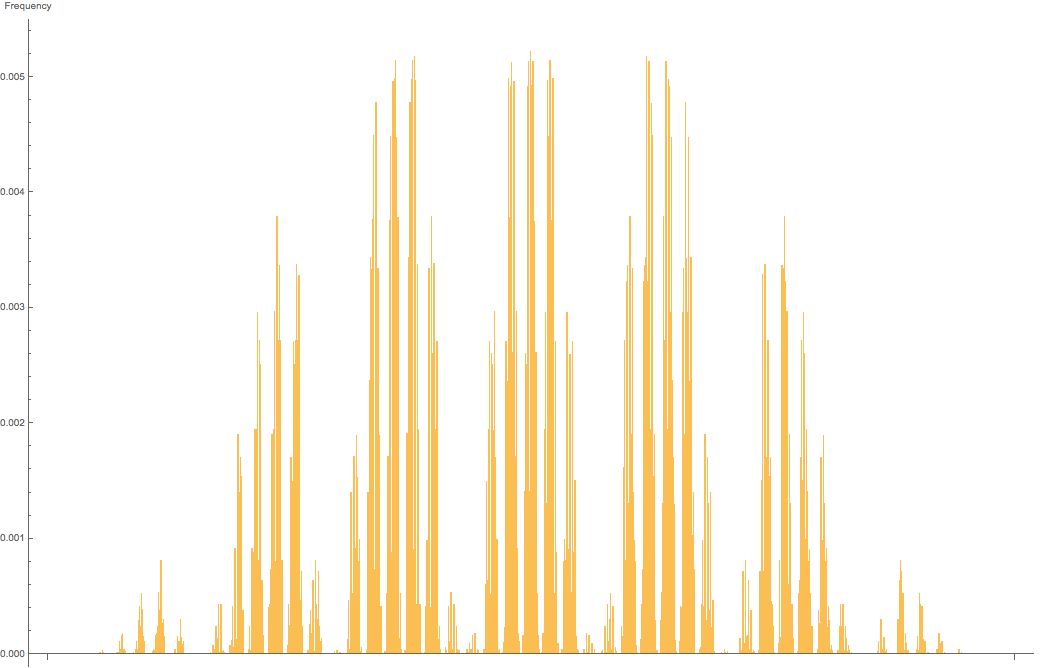
\includegraphics[width=0.65\textwidth]{RJs4square}
	\caption{\label{RJs4square}
$s=4$. Frequencies of $[2\!\times\!2]$ spatiotemporal domains.
            }
\end{figure}


\section{Summary}

The results obtained by simulations for the frequencies of words are
consistent with the unpublished B.~Gutkin analytical results. By
evaluating  analytical inequalities and finding the areas corresponding
to the frequencies of words of single cat map, we are able to find the
inadmissible sequences for words of up to length 6.

While for the \catlatt s the general inequalities can be stated for any
rectangular spatiotemporal domain, determining the volumes confined by these
inequalities remains an open problem.

\begin{figure}
	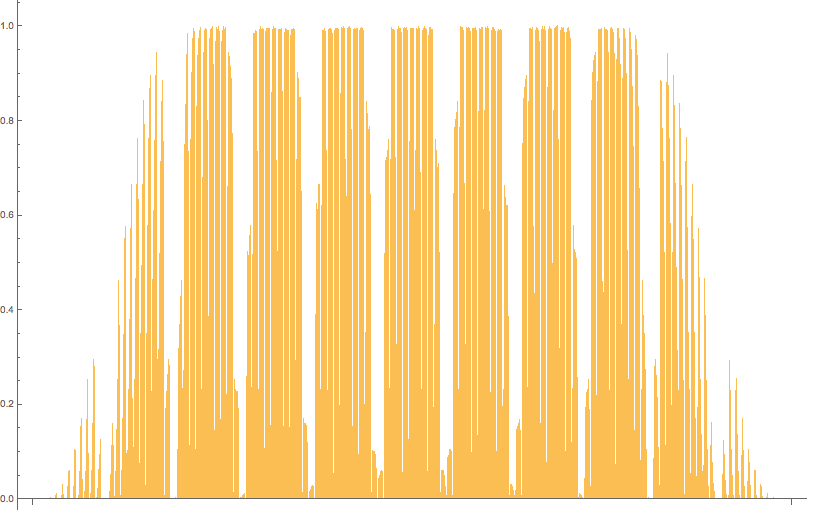
\includegraphics[width=0.65\textwidth]{RJs8square}
	\caption{\label{RJs8square}
$s=8$. Frequencies of $[2\!\times\!2]$ spatiotemporal domains.
            }
\end{figure}


\renewcommand{\cl}[1]{{\ensuremath{|#1|}}}  % the length of a periodic orbit, Ronnie
%%%%%%%%%%%%%%%%%%%%%%%%%%%%%%%%%%%%%%%%%%%%%%%%%%%%%%%%%%%%%%%%%%%%%%%
\printbibliography[heading=subbibintoc,title={References}]
